\chapter{Personen Profile}  % Kapitel % Steht dann über dem Text
\label{chapter:Personen Profile}  % Steht als Text im Inhaltsverzeichnis
\index{Personen Profile} % für das Stichwortverzeichnis

Jeder User der am CodeRed System registriert ist, hat ein eigenes Benutzerprofil. In diesem Benutzerprofil werden alle Daten zur Person angezeigt. Jeder User des Systems kann einsicht in das Profil anderer nehmen. \\
\\
Mentoren haben zusätzlich die Möglichkeit sich eine Liste der registrierten User anzeigen zu lassen. So haben sie leicht einen Überblick über alle aktiven User und können die passenden Einstufungen der User leicht vornehmen. \\
\\
Das Profil ist einfach aufgebaut und erhebt zwingende nur die Daten, die das System auch wirklich für einen reibungslosen Ablauf benötigt. Zwingend erforderlich sind Loginname, Name, Vorname und eine gültige E-Mail Adresse.\\
\\
\textbf{CodeRed und der Datenschutz?!} \\
CodeRed verfolgt grundsätzlich das Konzept der Datensparsamkeit. Das Projekt hält sich an das Deutsche sowie das Hessische Datenschutzgesetz. Das Sammeln unnötiger Daten oder sogar das weitergeben von Erhobenen Daten kommt für das Projekt CodeRed nicht infrage.
\footnote[1]{Datensparsamkeit ist ein Konzept im Bereich Datenschutz. Die Grundidee ist, dass bei der Datenverarbeitung nur soviele personenbezogene Daten gesammelt werden, wie für die jeweilige Anwendung unbedingt notwendig sind. Gerade das unkontrollierte Sammeln von sensitiven Daten durch öffentliche und nicht-öffentliche Stellen läuft dem Grundrecht auf informationelle Selbstbestimmung zuwider.\\
\\
Die Datensparsamkeit steht in engem Zusammenhang mit dem traditionellen datenschutzrechtlichen Grundsatz, dass nur diejenigen personenbezogenen Daten verarbeitet werden dürfen, die für die Erfüllung der jeweiligen Aufgabe benötigt werden (Erforderlichkeit). Sie ist jedoch auch ein Aspekt des Systemdatenschutzes, d.h. der Integration der Datenschutzanforderungen in die IT-Systeme. Datenschutz soll nicht allein durch gesetzliche Regelungen normiert sondern auch durch das Design der IT realisiert werden.\\ In Deutschland sind Datensparsamkeit und Datenvermeidung in § 3a BDSG als Ziel der Gestaltung und Auswahl von Datenverarbeitungssystemen festgeschrieben.}
\newpage
\begin{figure}[h]
\begin{center}
   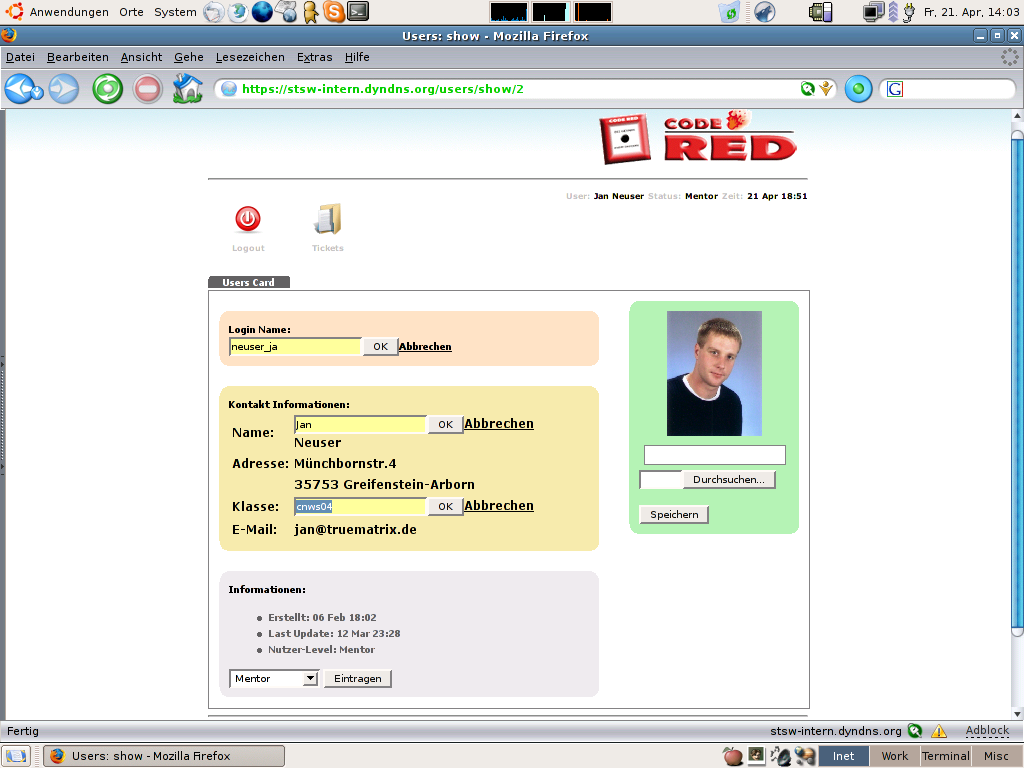
\includegraphics[width=450pt]{../bilder/profil_edit.png}
   \caption{Benutzer Profil}
   \label{Benutzer Profil}
\end{center}
\end{figure}
Um seine Einträge zu ändern, muss einfach nur auf die zu editirernde Stelle geklickt werden.\\
$($ Siehe Grafik$)$.\\
\\
Das Avatar soll Hauptsächlich zu bessern Erkennung von Personen und Orten im System dienen. Die Wiedererkennung ist so wesentlich größer und alle beteiligten an einem Ticket können sich so leichter identifizieren. Laden sie also Möglichst ein aktuelles Passbild von ihnen in ihr Benutzerprofil.\\
\\




   
